\chapter{Speichertechnologien}

Nach den Ladesystemen werden in diesem Kapitel nun die Energiespeicher für Stadtbusse betrachtet. Wie im vorigen Kapitel werden zunächst die Bewertungskriterien und die betrachteten Technologien erläutert. In Abschnitt \ref{vergleichstabellen_speichertechnologien} ab Seite \pageref{vergleichstabellen_speichertechnologien} werden die Werte aufgelistet.

Im Gegensatz zu den Ladesystemen ist die Produktvielfalt der Speichertechnologien nahezu unbegrenzt. Von daher können hier nicht alle Batterien verglichen werden, sondern es werden einzelne Produkte verglichen, die repräsentativ für die jeweilige Technologie sind.\marginpar{Wirklich?}

\section{Bewertungskriterien}
\marginpar{Wie wurde ausgewählt?\\
	       Saubere Definitionen}
Die Bewertungskriterien wurden ausgewählt, um neben den \emph{Kenndaten} die technischen Anforderungen von hoher \emph{Effizienz}, langer \emph{Lebensdauer} und \emph{Sicherheit} widerzuspiegeln. Bei verschiedenen Ladestrategien könen sich die Energiespciher unterschieldlich verhalten. Von daher wird bei einigen Kriterien zwischen \emph{Gelegenheitsladung} und \emph{Nachtladung} unterschieden.

\emph{Nachtladung} zeigt das Verhalten des Energiespeichers in einem Bus, der tagsüber 16 Stunden lang ohne Zwischenladen in Betrieb ist und dabei den Energiespeicher auf 20\% entlädt. Über Nacht im Depot wird der Energiespeicher über acht Stunden auf 100\% geladen.

\marginpar{Ist Tour der richtige Begriff? Es gibt den VBB GTFS Dump für exakte Daten, die muss man bloß rauskriegen}
\emph{Gelegenheitsladung} zeigt das Verhalten des Energiespeichers, wenn der Bus am Ende jeder Tour aufgeladen wird. Im Laufe von einer Stunde wird der Energiespeicher auf 50\% entladen und dann mit maximaler Geschwindigkeit auf 90\% Ladezustand aufgeladen. Es wurde nur eine Entladung vo 40\% der Gesamtkapazität gewählt, da der Bus im Falle eines defektes der Ladestation noch genug Energie zur Verfügung haben soll, um die Ladestation am anderen Ende der Strecke zu erreichen.

Diese Ladeprofile stellen Extremfälle dar, im realen Betrieb wird meist eine Kombination von Aufladung im Depot und Nachladen an den Endhaltestellen gewählt.

\subsection{Kenndaten}

\begin{description}
	\item[Zellenspannung] Die elektrische Spannung einer Zelle bei 100\% Ladezustand.\marginpar{Oder 0.2C oder 1C Last?}\\
	Einheit: $V$
	\item[Ladung] Der Bereich von Ladungen, mit denen die Batterie gefertigt werden kann.\\
	Einheit: $mAh$ \marginpar{oder $Ah$?}	
	\item[Balancing] Methode, durch die die Zellenspannungen angeglichen werden.\\
	Möglichkeiten: Überladen, separate Ansteuerung jeder Zelle
\end{description}

\subsection{Effizienz}
Die spezifischen Größen werden für einen gesamten Energiespeicher bestimmt, das Gehäuse und interne Verkabelung haben einen Einfluss auf diese Größen.
\begin{description}
	\item[Energiedichte, Gelegenheitsladung] Die mit dieser Technologie erreichbare Energiedichte, wenn der Energiespeicher in einer Stunde von 90\% auf 40\% entladen wird. Dies entspricht einer Entladung mit 0,5C\footnote{\emph{C} ist eine für Batterien übliche Einheit der Belastung. Sie ist definiert als $\frac{Strom\ (in\ A)}{Ladung\ (in\ Ah)}$}\\
	Einheit: $\frac{Wh}{l}$ \marginpar{$l$ oder $m^3$?}
	\item[Spezifische Energie, Gelegenheitsladung] Die mit dieser Technologie erreichbare Energiedichte, wenn der Energiespeicher in einer Stunde von 90\% auf 40\% entladen wird..\\
	Einheit: $\frac{Wh}{kg}$
	\item[Energiedichte, Nachtladung] Die mit dieser Technologie erreichbare Energiedichte, wenn der Energiespeicher in 16 Stunden auf 20\% entladen wird. Dies entspricht einer Entladung mit 0,05C\\
	Einheit: $\frac{Wh}{l}$
	\item[Spezifische Energie, Nachtladung] Die mit dieser Technologie erreichbare Energiedichte, wenn der Energiespeicher in 16 Stunden auf 20\% entladen wird.\\
	Einheit: $\frac{Wh}{kg}$
	\item[Leistungsdichte, kontinuierlich] Für die Berechnung wird die maximale Dauerleistung verwendet.\\
	Einheit: $\frac{W}{kg}$
	\item[Spezifische Leistung, kontinuierlich] Für die Berechnung wird die maximale Dauerleistung verwendet.\\
	Einheit: $\frac{W}{l}$
	\item[Leistungsdichte, Anfahren] Für die Berechnung wird die maximale Leistung verwendet, die bei 20\% Ladezustand für 30s erreicht werden kann.\marginpar{Warum 30s? Warum 20\% SOC?}\\
	Einheit: $\frac{W}{kg}$
	\item[Spezifische Leistung, Anfahren] Für die Berechnung wird die maximale Leistung verwendet, die bei 20\% Ladezustand für 30s erreicht werden kann.\\
	Einheit: $\frac{W}{l}$
	%\item[Innenwiderstand beim Laden] Mit dem Innenwiderstand kann der Energieverlust innerhalb der Batterie berechnet werden\\
	%Einheit: $\Omega$ \marginpar{Lieber Round-Trip-Effizienz KiBaM \cite{jongerden2008battery}.}
	%\item[Innenwiderstand beim Entladen] Einheit: $\Omega$
	\item[Effizienz, Gelegenheitsladung] Das Verhältnis zwischen verwendeter und abgerufener elektrischer Energie, wenn der Energiespeicher mit der maximalen Laderate auf von 40\% auf 90\% Ladezustand geladen wird und dann mit 0,5C auf 40\% Ladezustand entladen wird.\\
	Einheit: 1
	\item[Effizienz, Nachtladung] Das Verhältnis zwischen verwendeter und abrufbarer elektrischer Energie, wenn der Energiespeiche innerhalb von acht Stunden von 20\% Ladezustand auf 100\% Ladezustand aufgeladen wird und dann mit 0,05C auf 20\% Ladezustand entladen wird. Dies entspricht der Aufladung über Nacht im Depot oder der Aufladung von ausgewechselten Batterien in Batteriewechselsystemen.\\
	Einheit: 1
	\item[Nennladestrom] Der höchste Durchschnittliche Ladestrom, mit dem im Bereich zwischen 40\% und 90\% Ladezustand geladen werden kann\footnote{Der Kehrwert entspricht der Ladedauer zwischen 40\% und 90\% Ladezustand.}.\marginpar{Gleich den Kehrwert verwenden?}\\
	Einheit: $C\hat{=} \frac{Strom}{Ladung}$
\end{description}

\subsection{Lebensdauer und Sicherheit}
\begin{description}
	\item[Lebensdauer, kalendarisch] Die Zeitdauer, bis die Batterie nur noch 80\% der Anfangskapazität hat \cite{Sterner:2014}[S. 269]. \marginpar{Temperatur?}\\
	Einheit: $a$
	\item[Zyklenfestigkeit, Gelegenheitsladung] Die Anzahl an Ladezyklen in diesem Ladeprofil, bis die Batterie nur noch 80\% der Anfangskapazität hat. Ein Ladezyklus entspricht einer Auf- und Entladung um Nennkapazität\footnote{Also entspricht ein Ladezyklus \emph{zwei} Auf- und Entladungen zwischen 90\% und 40\%.}.\\
	Einheit: $1$
	\item[Zyklenfestigkeit, Nachtladung] Die Anzahl an Ladezyklen in diesem Ladeprofil, bis die Batterie nur noch 80\% der Anfangskapazität hat.\\
	Einheit: $1$
	\item[Zyklenfestigkeit, Nachtladung] 
	\item[Temperatur für thermisches durchgehen] Die Temperatur, ab dem eine weitere Temperaturerhöhung unumkehrbar ist.\\
	Einheit: $^\circ C$
\end{description}

\section{Betrachtete Technologien}
Im folgenden Abschnitt werden die Grundlagen und die Einsatzgeschichten der verschiedenen Speichertechnologien kurz erläutert. Die Technologien sind nach dem genutzten physikalischen Effekt aufgeteilt \cite{Sterner:2014}[S. 35f]. Im realen Betrieb werden manchmal auch Kombinationen von verschiedenen Speichertechnologien eingesetzt, um dem hohen Leistungsbedarf beim Anfahren und bei der Bremsenergierückgewinnung gerecht zu werden.

\subsection{Mechanisch – Schwungradspeicher}
In Bussen kann mechanische Energie mit einem Schwungrad gespeichert werden\footnote{Es gibt auch Prototypen von Pressluftspeichern in kleineren Fahrzeugen, in Bussen werden sie jedoch nur als Teil eines Hybridantriebs eingesetzt und hier nicht weiter betrachtet \cite{Sebastian-Naumann:2014}[S. 14].}. Die Energieübertragung erfolgt durch eine elektrische Motor- und Generatoreinheit. Moderne Schwungräder werden aus gewickelten Karbonfasern hergestellt und in Vakuumgehäusen magnetisch gelagert, sie erreichen hohe Drehzahlen und geringe Reibungsverluste \cite{993788}. Im Falle eines berstenden Schwungrades muss das Gehäuse die gesamte Energie innerhalb von Sekundenbruchteilen aufnehmen, ohne selbst zu bersten. Dies erfordert sehr schwere Gehäuse, die die spezifische Energie und Leistung eines tatsächlichen Systems stark reduzieren. Der Schwungradspeicher wurde in den fünfziger Jahren im Gyrobus im schweizerischen Yverdon auf einer acht Kilometer langen Linie erprobt. Die Strecke wurde erfolgreich zurückgelegt, die damalige Technologie war jedoch sehr wartungsaufwändig und weniger effizient als ein Oberleitungsbus. Aktuell wird der Schwungradspeicher nur als Teil eines hybriden Antriebsstrangs eingesetzt \cite{tub_aleph001746639}[S. 216].

\subsection{Elektrisch – Kondensator}
Der Kondensator ist ein rein elektrischer Energiespeicher. Im klassischen Plattenkondensator werden zwei durch einen festes Dielektrikum getrennte Platten elektrisch aufgeladen, die Ladung kann später in Strom umgewandelt werden. Kondensatoren haben eine hohe spezifische Leistung, aber eine sehr geringe spezifische Energie. In Bussen werden sogenannte Superkondensatoren verwendet, die statt eines festen Dielektrikums ein Elektrolyt (meist eine Salz-Wasser-Lösung) verwenden. Die im Elektrolyt gelösten Ionen werden von der geladenen Platte angezogen, können sie jedoch aufgrund der umgebenden Wasserschicht nicht erreichen (siehe Abbildung \ref{abb_doppelschicht}). Da der Abstand zwischen Platte un Ionen extrem klein ist, entsteht eine sehr hohe elektrische Kapazität. Eine weitere Kapazitätssteigerung wird durch die Einlagerung von einigen Elektronen des Elektrolyts in den Leiterplatten erreicht \cite{Sterner:2014}[S. 167f].

\begin{figure}\centering
	 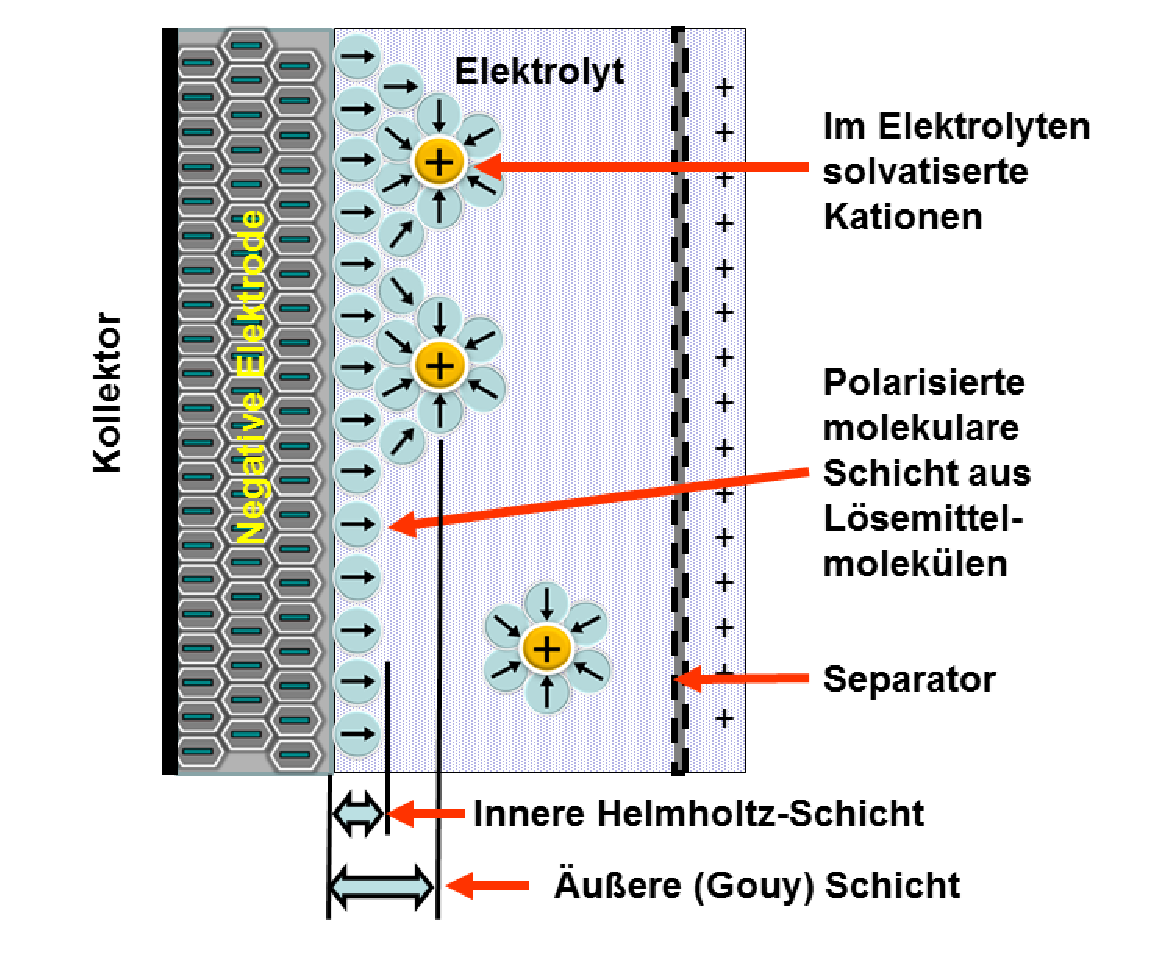
\includegraphics[width=\myFigureStandardWidth]{Doppelschicht-Prinzipdarstellung}
	 \caption{Prinzipdarstellung der Doppelschichtkapazität. Quelle: Elcap (Own work) CC BY-SA 3.0, via Wikimedia Commons}
	 \label{abb_doppelschicht}
\end{figure}

In Shanghai werden Busse mit dieser Technologie seit 2008 im Linienverkehr eingesetzt, daneben werden Superkondensatoren für kurzzeitige Einsätze mit hohem Leistungsbedarf, zum Beispiel zur Bremsenergierückgewinnung oder zur Überbrückung stromloser Stellen in Trolleybussen eingesetzt \cite{Barminer-Busgesellschaft:2012}.

\subsection{Elektrochemisch – Batterie} %TODO: Besser
Batterien bestehen aus zwei Elektroden aus meist verschiedenen Metallen. Zwischen den Elektroden befindet sich ein Elektrolyt, in dem sich Ionen von der einen Elektrode zur anderen bewegen können. Durch die Bewegung der Ionen wird Ladung übertragen und an den Klemmen der Batterie entsteht eine Spannung. Hier werden nur wiederaufladbare Batterien (sogenannte Sekundärbatterien) betrachtet\footnote{Die Begriffe Batterie, Akkumulator und Akku werden austauschbar verwendet.}, die für den Einsatz in Fahrzeugen geeignet sind. In der Herstellung werden einzelne Batteriezellen in parallel- und Reihenschaltung zu Batteriemodulen zusammengefasst, um höhere Ströme und Spannungen zu erreichen. Die Bauformen sind sehr unterschiedlich, meist werden jedoch gewickelte oder ineinander geschachtelte Flache Elektroden verwendet um die Oberflächen und damit die Stromstärke zu maximieren \cite{Sterner:2014}[S. 209ff].

\subsubsection{Blei-Säure}
Der Blei-Säure-Akkumulator besteht aus zwei Bleielektroden in einer Schwefelsäurelösung. Vor dem ersten Aufladen bildet sich an beiden Elektronen Bleisulfat ($PbSO_4$). Die Elektrodengleichungen sind in Tabelle \ref{Pb} aufgeführt \cite{KiehneBattery}[S. 50].

\begin{table}\centering
  \begin{tabularx}{\linewidth}{XrcX}
  	                   &                       $geladen$ & $\rightleftarrows$ & $entladen$             \\
  	Negative Elektrode & $PbO_2 + H_2SO_4 + 2H^+ + 2e^-$ & $\rightleftarrows$ & $PbSO_4 + 2H_2O$       \\
  	Positive Elektrode &                  $Pb + H_2SO_4$ & $\rightleftarrows$ & $PbSO_4 + 2H^+ + 2e^-$ \\ \midrule
  	Zellenreaktion     &         $Pb + PbO_2 + 2H_2SO_4$ & $\rightleftarrows$ & $2PbSO_4 + 2H_2O$      \\
  \end{tabularx}
  \caption{Elektrodengleichungen der Blei-Säure-Batterie}
  \label{Pb}
\end{table}

Im Gegensatz zu den meisten anderen Batterien transportiert hier der Elektrolyt nicht nur die Ionen, sondern ist selbst an der Reaktion beteiligt.

Im geladenen Zustand wird das enthaltene Wasser elektrolytisch zu Wasserstoff und Sauerstoff zerlegt. Dieser Wasserverlust muss durch periodisches Nachfüllen oder Rekombination der Gase zu Wasser ausgeglichen werden. Vorteil der Gasentwicklung ist, das so durch Überladen die Spannungen verschiedener Zellen angeglichen werden können, da die Energie des Überladevorgangs in die Wasserspaltung geführt wird \cite{tub_aleph001746639}[S. 182].

Der Blei-Säure-Akkumulator ist eine der ältesten wiederaufladbaren Batterietechnologien und wurde in allen frühen Elektrobussen eingesetzt, zum Beispiel im weltweit ersten Batteriebus, der ab 1900 auf der Strecke Anhalter Bahnhof – Stettiner Bahnhof (heute: Nordbahnhof) in Berlin erprobt wurde \cite{Risch:1957}[S. 8f].

\subsubsection{Nickel-Cadmium}
Die Elektroden bestehen aus Nickelhydroxid und Cadmiumhydroxid in einem alkalischen, wässrigen Elektrolyt, dass nicht an der Reaktion beteiligt ist, sondern nur dem Ionentransport dient. Die Reaktionsgleichungen sind in Tabelle \ref{NiCd} aufgeführt \cite{Sterner:2014}[S.233].

\begin{table}\centering
  \begin{tabularx}{\linewidth}{XrcX}
  	                   &               $geladen$ & $\rightleftarrows$ & $entladen$             \\
  	Negative Elektrode &            $Cd + 2OH^-$ & $\rightleftarrows$ & $Cd(OH)_2 + 2e^-$      \\
  	Positive Elektrode & $2NiOOH + 2H_2O + 2e^-$ & $\rightleftarrows$ & $2Ni(OH)_2 + 2OH^-$    \\ \midrule
  	Zellenreaktion     &   $Cd + 2NiOOH + 2H_2O$ & $\rightleftarrows$ & $Cd(OH)_2 + 2Ni(OH)_2$ \\
  \end{tabularx}
  \caption{Elektrodengleichungen der Nickel-Cadmium-Batterie}
  \label{NiCd}
\end{table}

Wie bei Blei-Säure-Batterien wird der Elektrolyt in Wasserstoff und Sauerstoff zerlegt, es sind offenen Bauformen und geschlossene Bauformen mit interner Rekombination vorhanden.

Die Nickel-Cadmium Batterie weist eine weit höhere spezifische Energie als die Blei-Säure-Batterie auf, wird jedoch in elektrischen Bussen nicht verwendet.

\subsubsection{Nickel-Metallhydrid}
Die Nickel-Metalhydridbatterie verwendet wie die Nickel-Cadmiumbatterie eine Nickel(oxy)hydroxidelektrode und einen alkalischen Elektrolyt. Der Unterschied ist, das hier statt giftigem Cadmium(hydroxid) in der negativen Elektrode Metall eingesetzt, in dem $H^+$-Ionen zu Wasserstoff reduziert und eingelagert werden. Dieser Hydrierung genannte Vorgang tritt in vielen verschiedenen Metallen und Legierungen auf. In diesen Batterien wird meist eine Legierung aus seltenen Erden und Nickel verwendet \cite{KiehneBattery}[S. 85ff]. Die Reaktionsgleichungen sind in Tabelle \ref{NiMH} aufgeführt \cite{Sterner:2014}[S. 245].

\begin{table}\centering
  \begin{tabularx}{\linewidth}{XrcX}
  	                   &              $geladen$ & $\rightleftarrows$ & $entladen$        \\
  	Negative Elektrode &          $M(H) + OH^-$ & $\rightleftarrows$ & $M + H_2O + e^-$  \\
  	Positive Elektrode &   $NiOOH + H_2O + e^-$ & $\rightleftarrows$ & $Ni(OH)_2 + OH^-$ \\ \midrule
  	Zellenreaktion     & $M(H) + NiOOH + 2H_2O$ & $\rightleftarrows$ & $M + Ni(OH)_2$    \\
  \end{tabularx}
  \caption{Elektrodengleichungen der Nickel-Metallhydrid-Batterie}
  \label{NiMH}
\end{table}

Da die Hydrierung bei Drücken von bis zu 10 Bar stattfindet, gibt es nur geschlossene Bauformen. Der Nickel-Metallhydrid-Akku wird in mehreren Hybridfahrzeugen verwendet, zum Beispiel im Toyota Prius.

\subsubsection{Lithium-Ionen}
In Lithium-Ionen-Akkus erfolgt der Ladungstransfer durch $Li^+$-Ionen, die durch ein Elektrolyt aus Lithiumsalzen in organischen Lösungsmitteln wandern. Der Elektrolyt ist häufig in ein Polymer eingelagert, das so entstandene Gel dient sowohl als Elektrolyt als auch zur mechanischen Separation der Elektroden\footnote{Es wird auch an einphasigen, festen Polymerelektrolyten geforscht, mit deren geringer Dicke eine hohe Energiedichte erreicht werden könnte. Diese Technologie wird jedoch noch nicht kommerziell eingesetzt.} \cite{xu2004nonaqueous}. Im Gegensatz zu den anderen Batterietypen, bei denen das Elektrodenmaterial oxidiert und reduziert wird, wandert hier das Metall selber von Elektrode zu Elektrode. Reine Lithiumelektroden würden sich auflösen und dadurch ihre Form verlieren, von daher werden für positive und negative Elektrode verschiedene Materialien verwendet, in denen die Lithiumionen eingelagert werden \cite{KiehneBattery}[S. 408, 440ff].

\paragraph{Geschichtete Oxide}

\begin{figure}\centering
	 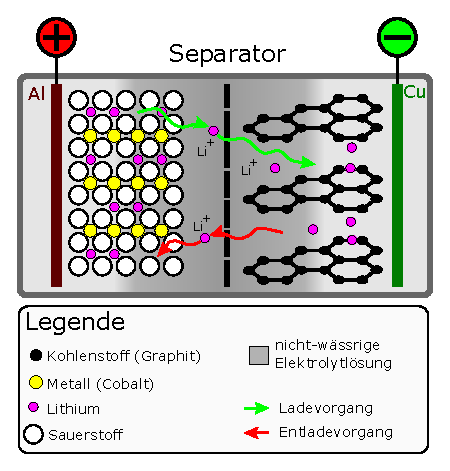
\includegraphics[width=\myFigureStandardWidth]{LiCoO2}
	 \caption{Prinzipdarstellung eines Lithium-Ionen-Akkus mit Kobaltoxid in der positiven Elektrode. Quelle: Cepheiden (Own work) CC BY-SA 2.0, via Wikimedia Commons}
	 \label{abb_LiCoO2}
\end{figure}

In kleinen und mittelgroßen Akkus werden meist positive Elektroden aus Lithium-Metalloxiden verwendet. Diese haben eine kubische Kristallstruktur, das Lithium wird zwischen den Sauerstoffatomen eingelagert. Positive Elektroden aus $LiCoO_2$ werden seit den 90er Jahren in kommerziellen Lithiumakkus verwendet. Daneben werden auch $LiMn_2O_4$, und $LiMnO_2$ verwendet, mit denen man günstigere Akkus auf Kosten der spezifischen Energie herstellen kann \cite{whittingham2004lithium}. %TODO: Welche Busse?

Die negative Elektrode besteht in allen Fällen aus Graphit, die Lithiumionen werden zwischen den verschiedenen Schichten der Graphitkristalle eingelagert. Es werden verschiedene Größen von Graphitkristallen und auch andere Modifikationen von Kohlenstoff verwendet \cite{Sterner:2014}[S. 252]. Ein Lithium-Kobaltoxid-Akku ist in Abbildung \ref{abb_LiCoO2} schematisch dargestellt.

\paragraph{Lithium-Eisenphosphat}
Lithium-Eisenphosphat ($LiFePO_4$) ist ein neues Material für die positive Elektrode. Die theoretische spezifische Energie ist ähnlich der von geschichteten Oxiden, aktuell wird jedoch nur eine niedrigere spezifische Energie erreicht \cite{Tie201382}. In der negativen Elektrode wird Graphit verwendet. Aufgrund des niedrigen Preises von Eisen sind diese Batterien gut für elektrische Fahrzeuge geeignet und werden zum Beispiel in den elektrischen Bussen von \textsc{BYD} verwendet \cite{bydSpecs}.

\paragraph{Lithium-Titanat}
Im Gegensatz zu den vorigen Materialien ist Lithium-Titanat ($Li_4Ti_5O_{12}$) kein Material für die positive Elektrode, sondern ersetzt das Graphit in der negativen Elektrode und wird meist in Kombination mit $LiCoO_2$ eingesetzt. Diese Technologie bietet eine niedrigere spezifische Energie, dafür eine weit höhere spezifische Lade- und Entladeleistung \cite{veneri2012charging}. Damit ist sie insbesondere für Stadtbusse mit Gelegenheitsladung interessant und wird zum Beispiel von \textsc{Proterra} in elektrischen Stadtbussen eingesetzt \cite{protCat}.

\subsubsection{Natrium-Nickelchlorid}
Die Natrium-Nickelcloridbatterie (auch als ZEBRA-Batterie bekannt) ist eine Hochtemperaturbatterie. Sie verwendet als Elektrolyt feste Alumiumkeramik, die nur für $Na^+$-Ionen durchlässig ist. Die Elektroden bestehen aus flüssigem Kochsalz und Nickel, der ebenfalls in flüssigem Kochsalz gelagert ist. Die Reaktionsgleichungen sind in Tabelle \ref{ZEBRA} aufgeführt \cite{KiehneBattery}[S. 257ff].

\begin{table}\centering
  \begin{tabularx}{\linewidth}{XrcX}
  	                   &       $geladen$ & $\rightleftarrows$ & $entladen$           \\
  	Negative Elektrode & $NiCl_2 + 2e^-$ & $\rightleftarrows$ & $2Cl^- + 2Na^+ + Ni$ \\
  	Positive Elektrode &           $2Na$ & $\rightleftarrows$ & $2e^-$               \\ \midrule
  	Zellenreaktion     &  $2Na + NiCl_2$ & $\rightleftarrows$ & $Ni + 2NaCl$
  \end{tabularx}
  \caption{Elektrodengleichungen der Natrium-Nickelchlorid-Batterie}
  \label{ZEBRA}
\end{table}

Damit das Kochsalz flüssig bleibt, muss die Batterie permanent geheizt werden, es werden immer ca. 100W pro 20kWh Kapazität zum Heizen benötigt. Im Gegenzug besitzt dieser Batterietyp eine hohe Lebensdauer und Leistungsdichte. In Kalifornien wurde ein Schulbus mit dieser Batterietechnologie erprobt \cite{Electric-Transportation-Department:2004}.

\section{Vergleichstabellen}
\label{vergleichstabellen_speichertechnologien}
\marginpar{Mehr Daten\\
	       saubere Quellen}
\begin{table}\centering
	\begin{tabularx}{\linewidth}{lXXX}
		\toprule
		\multirow{2}{*}{Technologie} & Zellenspannung           & Ladung       & Balancing \\
		                             & $V$                      & $mAh$        & $ $       \\ \midrule
		\textbf{Mechanisch}          &                          &              &  \\
		Schwungrad                   & k. A.                    & k. A.        & k. A.     \\
		\textbf{Elektrostatisch}     &                          &              &  \\
		Superkondensator             & ???                      & ???          & ???       \\
		\textbf{Elektrochemisch}     &                          &              &  \\
		Blei-Säure                   & 2,1 \cite{Sterner:2014}  & ???          & Überladen \\
		Nickel-Cadmium               & 1,35 \cite{Sterner:2014} & ???          & Überladen \\
		Nickel-Metallhydrid          & 1,35 \cite{Sterner:2014} & ???          & Überladen \\
		Li-Ion -- $LiCoO_2$          & 4? \cite{Sterner:2014}   & ???          & Balancer  \\
		Li-Ion -- $LiFePO_4$         & 3,2? \cite{Sterner:2014} & 2000 -- 4500 & Balancer  \\
		Li-Ion -- $Li_4Ti_5O_{12}$   & 2,6? \cite{Sterner:2014} & 4000         & Balancer  \\
		Ni-NaCl (ZEBRA)              & 2,58 \cite{Sterner:2014} & ???          & ???       \\ \bottomrule
	\end{tabularx}
	\caption{Kenndaten der Energiespeicher}
\end{table}

\begin{table}\centering
	\begin{tabularx}{\linewidth}{lllll}
		\toprule
		\multirow{2}{*}{Technologie} & Energiedichte  & Spez. Energie   & Leistungsdichte & Spez. Leistung \\
		                             & $\frac{Wh}{l}$ & $\frac{Wh}{kg}$ & $\frac{W}{l}$   & $\frac{W}{kg}$ \\ \midrule
		\textbf{Mechanisch}          &                &                 &                 &  \\
		Schwungrad                   & ???            & ???             & ???             & ???            \\
		\textbf{Elektrostatisch}     &                &                 &                 & ?              \\
		Superkondensator             & ???            & ???             & ???             & ???            \\
		\textbf{Elektrochemisch}     &                &                 &                 &  \\
		Blei-Säure                   & ???            & ???             & ???             & ???            \\
		Nickel-Cadmium               & ???            & ???             & ???             & ???            \\
		Nickel-Metallhydrid          & ???            & ???             & ???             & ???            \\
		Li-Ion -- $LiCoO_2$          & ???            & ???             & ???             & ???            \\
		Li-Ion -- $LiFePO_4$         & ???            & ???             & ???             & ???            \\
		Li-Ion -- $Li_4Ti_5O_{12}$   & ???            & ???             & ???             & ???            \\
		Ni-NaCl (ZEBRA)              & ???            & ???             & ???             & ???            \\ \bottomrule
		                             &
	\end{tabularx}
	\caption{Spezifische Größen der Energiespeicher}
	\label{hierdoof}
\end{table}
\marginpar{Typografie ist in \ref{hierdoof} doof}
\marginpar{Layout: Die Tabellen müssen irgendwie anders sortiert werden…}

\begin{table}\centering
	\begin{tabularx}{\linewidth}{XXXX}
		\toprule
		\multirow{2}{*}{Technologie} & Kal. Lebensdauer & Zyklenfestigkteit & Max. Temperatur \\
		                             & a                        & 1                 & $^\circ C$      \\ \midrule
		\textbf{Mechanisch}          &                          &                   &  \\
		Schwungrad                   & ???                      & ???               & ???             \\
		\textbf{Elektrostatisch}     &                          &                   &  \\
		Superkondensator             & ???                      & ???               & ???             \\
		\textbf{Elektrochemisch}     &                          &                   &  \\
		Blei-Säure                   & ???                      & ???               & ???             \\
		Nickel-Cadmium               & ???                      & ???               & ???             \\
		Nickel-Metallhydrid          & ???                      & ???               & ???             \\
		Li-Ion -- $LiCoO_2$          & ???                      & ???               & ???             \\
		Li-Ion -- $LiFePO_4$         & ???                      & ???               & ???             \\
		Li-Ion -- $Li_4Ti_5O_{12}$   & ???                      & ???               & ???             \\
		Ni-NaCl (ZEBRA)              & ???                      & ???               & ???             \\ \bottomrule
		                             &
	\end{tabularx}
	\caption{Lebensdauer und Sicherheit der Energiespeicher}
\end{table}
